\documentclass[12pt]{article}

\usepackage{pablo-devoir}
\usepackage[a5paper,margin=1cm]{geometry}

\pagestyle{empty}

\title{Lecture graphique d'équations de fonctions affines}
\date{}
\classe{2\up{des}}
\dsnum{}

\newcommand{\affine}[5]{
    \draw[dotted,color=gray] (#1,#2) grid (#3,#4);
    \draw[-latex] (#1,0) -- (#3,0);
    \draw[-latex] (0,#2) -- (0,#4);
    \draw (0,0) node[below left]{$\mathcal{O}$};
    \draw (1,0) node[below]{$I$};
    \draw (0,1) node[left]{$J$};

    \foreach \xstart/\xend/\a/\b in {#5} {
      \draw[smooth,blue,domain=\xstart:\xend] plot ({\x},{\a*\x+\b});
    }
}

\begin{document}

\maketitle

\section{Méthode}

\begin{center}
  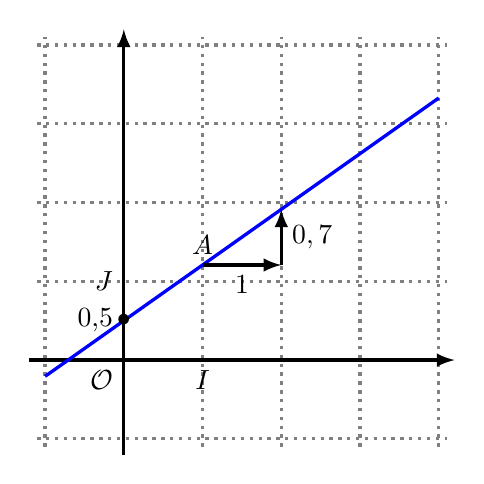
\begin{tikzpicture}[very thick, domain=-1:4]
    \draw[dotted,color=gray] (-1.1,-1.1) grid (4.1,4.1);
    \draw[-latex] (-1.2,0) -- (4.2,0);
    \draw[-latex] (0,-1.2) -- (0,4.2);
    \draw (0,0) node[below left]{$\mathcal{O}$};
    \draw (1,0) node[below]{$I$};
    \draw (0,1) node[left]{$J$};
    \draw[smooth,blue] plot ({\x},{sqrt(2)*\x/2+0.5});

    \draw[-latex] (1, {sqrt(2)/2+0.5}) node[above]{$A$} -- ++(1,0) node[midway, below]{1};
    \draw[-latex] (2, {sqrt(2)/2+0.5}) -- ++(0, {sqrt(2)/2}) node[midway,right]{$0,7$};

    \draw (0,0.5) node{$\bullet$} node[left]{0,5};
  \end{tikzpicture}
\end{center}

  \paragraph{Coefficient directeur}
  \begin{enumerate}
    \item On choisit un point quelconque sur la droite (par exemple $A$).
    \item Partant de $A$, on trace un segment horizontal, vers la droite, d'une unité.
    \item On trace ensuite un segment, vertical, jusqu'à rencontrer la droite.
    \item On mesure la longueur de ce segment vertical : c'est le coefficient directeur, auquel il manque (éventuellement) le signe.
    \item Si la fonction est croissante, le coefficient directeur est positif, sinon, il est négatif.
  \end{enumerate}

  \paragraph{Ordonnée à l'origine}
  On lit l'ordonnée du point d'intersection de la droite avec l'ordonnée.

  \paragraph{Bilan}
  En appliquant cette méthode à l'exemple, on obtient : $f:x\mapsto 0,7x+0,5$.

  \section{Exercices}

Dans chaque cas, déterminer l'équation des fonctions affines représentées graphiquement. Les solutions sont données en fin de document.

  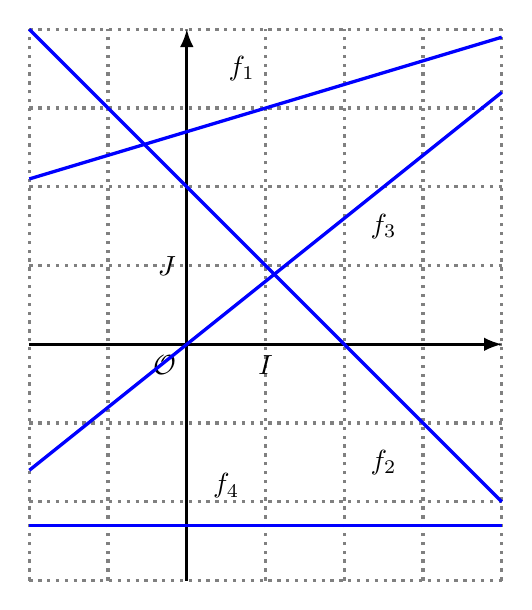
\begin{tikzpicture}[very thick]
  \affine{-2}{-3}{4}{4}{
    -2/4/0/-2.3,
    -2/4/-1/2,
    -2/4/.3/2.7,
    -2/4/.8/0
  }
  \draw (1, 3.5) node[left]{$f_1$};
  \draw (2.5, -1.5) node[]{$f_2$};
  \draw (2.5, 1.5) node[]{$f_3$};
  \draw (0.5, -1.8) node[]{$f_4$};
  \end{tikzpicture}
  \hfill
  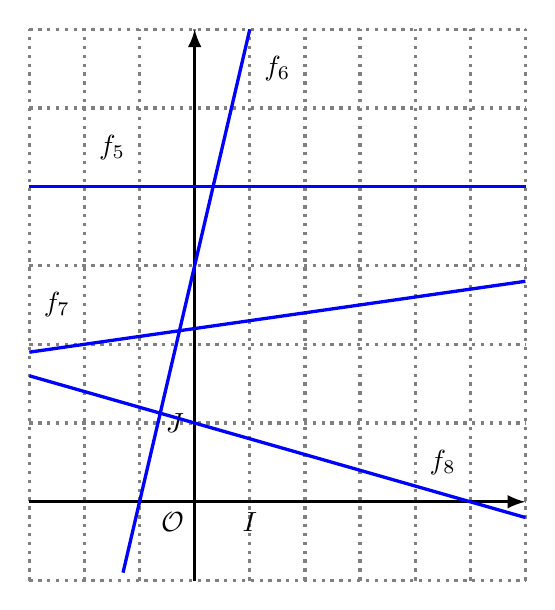
\begin{tikzpicture}[very thick,xscale=.7]
  \affine{-3}{-1}{6}{6}{
    -1.3/1/3/3,
    -3/6/-.2/1,
    -3/6/.1/2.2,
    -3/6/0/4
  }
  \draw (-1.5, 4.5) node[]{$f_5$};
  \draw (1.5, 5.5) node[]{$f_6$};
  \draw (-2.5, 2.5) node[]{$f_7$};
  \draw (4.5, .5) node[]{$f_8$};
  \end{tikzpicture}

  \section{Solutions}

  Ce sont des lectures graphiques, donc des solutions approchées. Si vos solutions sont \emph{à peu près} égales à celles trouvées ici, c'est que vous ne vous êtes pas trompés.

  \begin{align*}
    f_1:x&\mapsto 0,3x+2,7\\
    f_2:x&\mapsto -1x+2\\
    f_3:x&\mapsto 0,8x\\
    f_4:x&\mapsto -2,3\\
    f_5:x&\mapsto 4\\
    f_6:x&\mapsto 3x+3\\
    f_7:x&\mapsto 0,1x+2,2\\
    f_8:x&\mapsto -0,2x+1\\
  \end{align*}

\end{document}
